\chapter{Regression}

% ---------- MAE ----------
\clearpage
\thispagestyle{customstyle}
\section{MAE}
\subsection{Mean Absolute Error}

% ---------- MSE ----------
\clearpage
\thispagestyle{customstyle}
\section{MSE}
\subsection{Mean Squared Error}

% ---------- MSLE ----------
\clearpage
\thispagestyle{customstyle}
\section{MSLE}
\subsection{Mean Squared Log Error}

% ---------- RMSE ----------
\clearpage
\thispagestyle{customstyle}
\section{RMSE}
\subsection{Root Mean Squared Error}

% ---------- RMSLE ----------
\clearpage
\thispagestyle{customstyle}
\section{RMSLE}
\subsection{Root Mean Squared Log Error}

% ---------- MAPE ----------
\clearpage
\thispagestyle{customstyle}
\section{MAPE}
\subsection{Mean Absolute Percentage Error}

% ---------- sMAPE ----------
\clearpage
\thispagestyle{customstyle}
\section{sMAPE}
\subsection{Symmetric Mean Absolute Percentage Error}

% ---------- wMAPE ----------
\clearpage
\thispagestyle{customstyle}
\section{wMAPE}
\subsection{Weighted Mean Absolute Percentage Error}

% ---------- MASE ----------
\clearpage
\thispagestyle{customstyle}
\section{MASE}
\subsection{Mean Absolute Scaled Error}

% ---------- MSPE ----------
\clearpage
\thispagestyle{customstyle}
\section{MSPE}
\subsection{Mean Squared Prediction Error}

% ---------- MDA ----------
\clearpage
\thispagestyle{customstyle}
\section{MDA}
\subsection{Mean Directional Accuracy}

% ---------- MAD ----------
\clearpage
\thispagestyle{customstyle}
\section{MAD}
\subsection{Mean Absolute Deviation}

% ---------- MPD ----------
\clearpage
\thispagestyle{customstyle}
\section{MPD}
\subsection{Mean Poisson Deviance}

% ---------- MGD ----------
\clearpage
\thispagestyle{customstyle}
\section{MGD}
\subsection{Mean Gamma Deviance}

% ---------- R-squared ----------
\clearpage
\section{$\mathbf{R^2}$}
\subsection{R-squared}
\thispagestyle{customstyle}

R-squared needs little introduction; it's featured in every statistics book. Also known as the coefficient of determination, it's commonly introduced as a measure that quantifies the amount of variability explained by the regression model.

\begin{center}
\tikz{
\node[inner sep=2pt, font=\Large] (a) {
{
$\displaystyle
R^2 = 1 - \frac{\sum_{t=1}^n (Y_t - {\color{violet!50!blue}\hat{Y}_t})^2}{\sum_{t=1}^n ({\color{cyan}Y_t} - {\color{teal!70!green}\bar{Y}})^2}
$
}
};

\draw[-latex,violet!50!blue, semithick] ($(a.north)+(2.1,0)$) to[bend left=15] node[pos=1, right] {Predicted value} +(1,.5); 
\draw[-latex,teal!70!green, semithick] ($(a.south)+(2.1,0.1)$) to[bend right=15] node[pos=1, right] {Mean of targets} +(1,-.5); 
\draw[-latex,cyan, semithick] ($(a.south)+(1,0.1)$) to[bend left=15] node[pos=1, left] {Target value} +(-1,-.5); 
}
\end{center}

However, it may be easier to think of R-squared as a way to scale MSE between a perfect model and one that always predicts the mean. A score of 1.0 means $Y_t$ and $\hat{Y}_t$ are equal. Despite its name, R-squared can be negative if the model performs worse than just predicting the mean.

\textbf{When to use R-squared?}

R-squared can be more intuitive than MAE, MSE, RMSE, and other scale-dependent metrics since it can be expressed as a percentage, whereas the latter have arbitrary ranges.

\coloredboxes{
\item Easy Interpretation. Especially when interpreted as a scaled MSE.
\item R-squared is widely accepted in statistical analysis and research, making it a standard choice for evaluating model performance.
}
{
\item Just like MSE, R-squared can be sensitive to outliers, as large errors have a greater impact.
\item Be cautious about which value of $\bar{Y}$ to use. Most implementations default to $\bar{Y}_{\text {test }}$ which can lead to information leakage. It is advisable to use $\bar{Y}_{\text {train }}$ instead.
}


\clearpage
\thispagestyle{customstyle2}


\begin{figure*}[ht!]
    \centering
    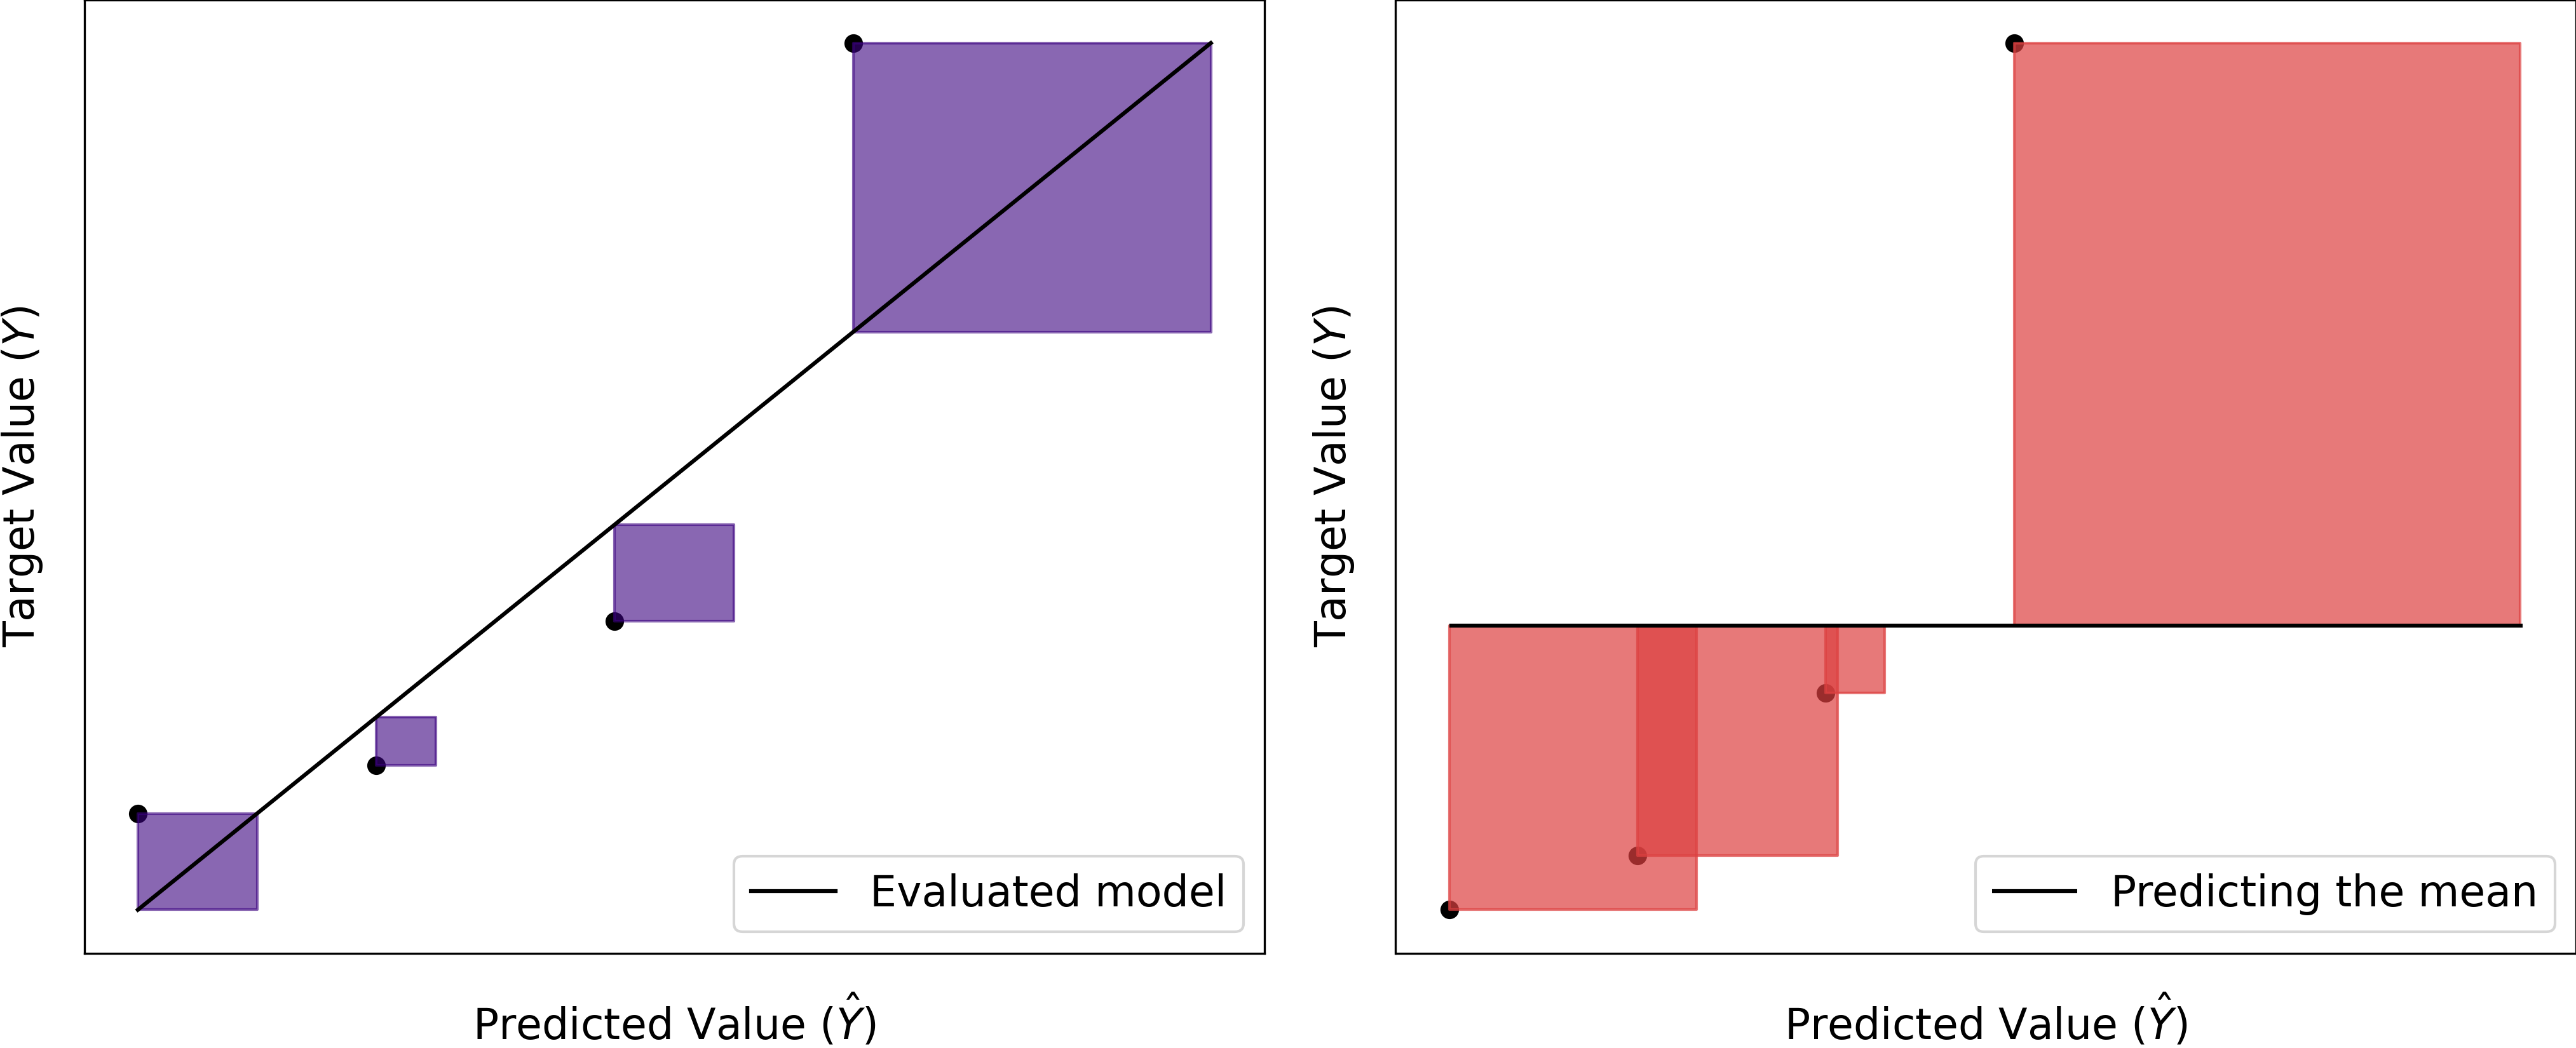
\includegraphics[width=\textwidth]{figures/R2_explained.png}
    % \caption{Caption}
    \label{fig1}
\end{figure*}

\begin{wrapfigure}{r}{0.5\textwidth}
    \centering
    \vspace{-10pt} % Adjust vertical alignment if needed
    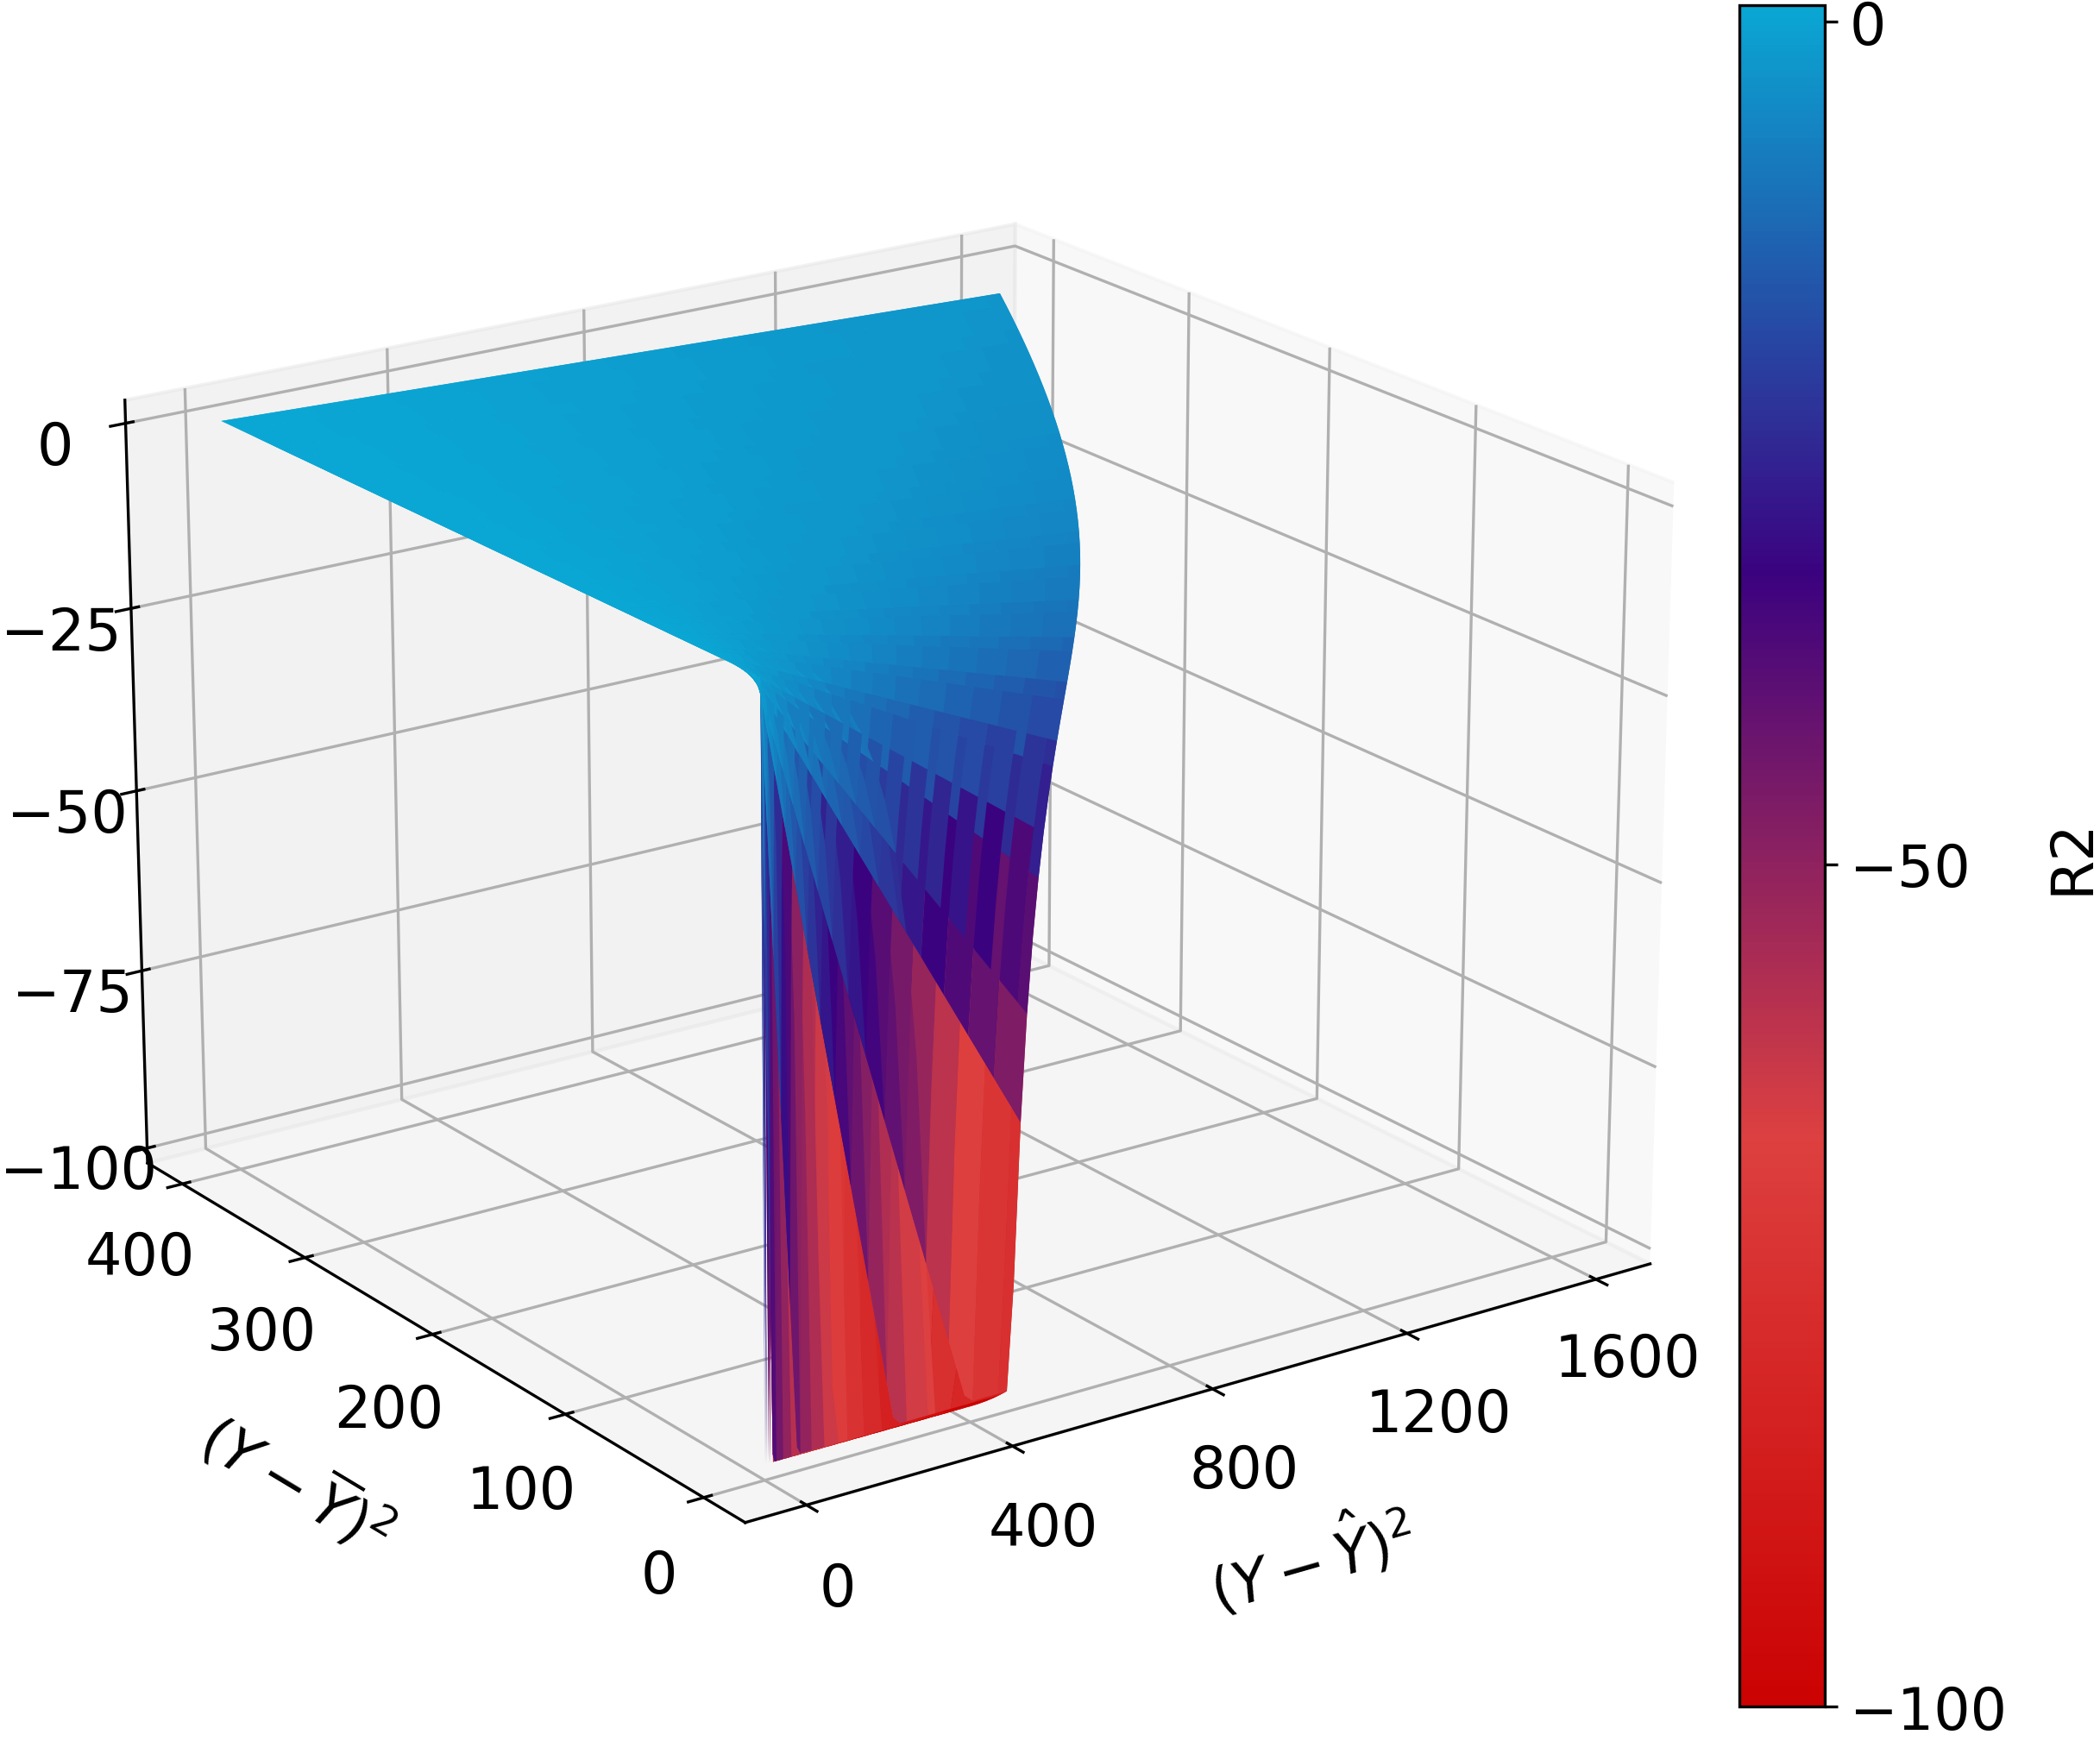
\includegraphics[width=0.45\textwidth]{figures/R2_3d_surface.png} % Your figure goes here
    \vspace{-10pt} % Adjust vertical alignment if needed
\end{wrapfigure}

% Left text with the image on the right
\textbf{Figure 2.15 R-Squared.} \textbf{Top:} The
areas of the purple squares
represent the MSE of the
evaluated model. While, the areas
of the red squares represent the
MSE of a model that always
predicts the mean. R-squared
can be written as $R^2 = 1-\frac{\color{violet!50}MSE_{model}}{\color{red!50}MSE_{baseline}}$\\
\textbf{Right:} R-squared quickly drops
into the negative region in cases
where the mean is a better
predictor than the evaluated
model.


\orangebox{%
Did you know that...}
{
R-squared is more than 100 years old; it was introduced by geneticist Sewall Wright in 1921.
}


\textbf{R-squared alternatives and other metrics to look for}

Other metrics commonly explored alongside R-squared are Adjusted Rsquared, out-of-sample R-squared, Mean Absolute Error (MAE), Mean Squared Error (MSE), Root Mean Squared Error (RMSE), etc.



% ---------- D2 ----------
\clearpage
\thispagestyle{customstyle}
\section{D2}
\subsection{D2 Absolute Score}

% ---------- Explained Variance Score ----------
\clearpage
\thispagestyle{customstyle}
\section{Explained Variance Score}
\subsection{Explained Variance Score}